%! Author = omar.iskandarani
%! Date = 5/28/2025


\section{Inleiding}
Het standaardmodel kan worden geherformuleerd via fundamentele constanten van het Vortex Æther Model (VAM). Alle interacties en deeltjes worden dan beschreven vanuit vloeistofachtige bewegingen en topologische structuren. De essentiële VAM-constanten zijn:
\begin{itemize}
    \item $C_e$: tangentiële snelheid in de wervelkern
    \item $r_c$: minimale kernstraal (circulatieschaal)
    \item $\rho_\text{\ae}$: ætherdichtheid
    \item $F_\text{max}$: maximale ætherkracht
\end{itemize}

\subsection*{Grootheden in VAM-Eenheden}
\begin{table}[h!]
    \centering
    \begin{tabular}{|c|l|}
        \hline
        \textbf{Symbool} & \textbf{Beschrijving} & \textbf{Eenheid in VAM} \\
        \hline
        $L_0$ &= $r_c$ & $\text{(lengte)}$ \\
        $T_0 $&=$ \frac{r_c}{C_e} $&$\text{(tijd)}$ \\
        $M_0$ &= $\frac{F_\text{max} r_c}{C_e^2}$ &$\text{(massa)}$ \\
       $ E_0$ &=$ F_\text{max} r_c $&$\text{(energie)}$
        \hline
    \end{tabular}
    \caption{Basisgrootheden in Vortex Æther Model.}
\end{table}


\begin{table}[h!]
    \centering
    \begin{tabular}{|c|l|l|}
        \hline
        \textbf{Symbool} & \textbf{Beschrijving} & \textbf{Eenheid in VAM} \\
        \hline
        $C_e$ & Tangentiële wervelsnelheid & $[L/T]$ \\
        $r_c$ & Kernstraal van wervel & $[L]$ \\
        $\rho_\text{\ae}$ & Ætherdichtheid & $[M/L^3]$ \\
        $F_\text{max}$ & Maximale kracht æther & $[M \cdot L/T^2]$ \\
        $\Gamma$ & Circulatie & $[L^2/T]$ \\
        $\hbar_\text{VAM}$ & Wervelmoment & $[M \cdot L^2 / T]$ \\
        $E_0$ & Elementaire energie & $[M \cdot L^2 / T^2]$ \\
        $T_0$ & Elementaire tijd & $[T]$ \\
        $L_0$ & Elementaire lengte & $[L]$ \\
        $M_0$ & Elementaire massa & $[M]$ \\
        \hline
    \end{tabular}
    \caption{Fundamentele grootheden in Vortex Æther Model.}
\end{table}

\begin{table}[H]
    \centering
    \caption{Derived Constants and Couplings in the Vortex Æther Model (VAM)}
    \begin{tabular}{|c|c|l|}
        \hline
        \textbf{Symbol} & \textbf{Expression} & \textbf{Interpretation} \\
        \hline
        $\hbar_\text{VAM}$ & $m_e C_e r_c$ & VAM analogue of the reduced Planck constant \\
        \hline
        $c$ & $\sqrt{\dfrac{2 F_\text{max} r_c}{m_e}}$ & Emergent wave speed (effective speed of light) \\
        \hline
        $\alpha$ & $\dfrac{2 C_e}{c}$ & Fine-structure constant (geometric formulation) \\
        \hline
        $e^2$ & $8\pi m_e C_e^2 r_c$ & Squared elementary charge in natural units \\
        \hline
        $\Gamma$ & $2\pi r_c C_e = \dfrac{h}{m_e}$ & Circulation quantum / quantized angular momentum \\
        \hline
        $v$ & $\sqrt{\dfrac{F_\text{max} r_c^3}{C_e^2}}$ & Higgs-like vacuum field amplitude in VAM \\
        \hline
    \end{tabular}
    \label{tab:VAM_constants}
\end{table}



\subsection*{Reformulated Lagrangian in VAM Units}
The full Lagrangian in the Vortex Æther Model (VAM) formulation reads:
\begin{align*}
    \mathcal{L}_\text{VAM} &=
    \underbrace{-\frac{1}{4} \sum_{a} F^{a}_{\mu\nu} F^{a\mu\nu}}_{\text{Gauge field kinetic term}} \\
    &+ \underbrace{\sum_{f} i \hbar_\text{VAM} \, \bar{\psi}_f \gamma^\mu D_\mu \psi_f}_{\text{Fermion kinetic term with } \hbar_\text{VAM} = m_f C_e r_c} \\
    &- \underbrace{\left| D_\mu \phi \right|^2}_{\text{Higgs kinetic term}} \\
    &- \underbrace{V(\phi)}_{\text{Higgs potential}}
    \qquad \text{with } V(\phi) = -\frac{F_\text{max}}{r_c}|\phi|^2 + \lambda |\phi|^4 \\
    &- \underbrace{\sum_f \left(y_f \bar{\psi}_f \phi \psi_f + \text{h.c.}\right)}_{\text{Yukawa couplings}} \\
    &+ \underbrace{\mathcal{H}_\text{topo}}_{\text{Topological helicity terms}}
\end{align*}

\begin{table}[H]
    \centering
    \caption{Interpretation of terms in the reformulated VAM Lagrangian}
    \label{tab:lagrangian_terms_vam}
    \begin{tabular}{|l|p{10cm}|}
        \hline
        \textbf{Term} & \textbf{Interpretation} \\
        \hline
        $F_{\mu\nu}^a$ & Field strength tensor of the gauge field (electroweak and color interactions). \\
        \hline
        $\bar{\psi}_f \gamma^\mu D_\mu \psi_f$ & Dirac term for fermions, where mass enters via $\hbar_\text{VAM} = m_f C_e r_c$. \\
        \hline
        $|D_\mu \phi|^2$ & Kinetic term of the Higgs field with gauge covariant derivative. \\
        \hline
        $V(\phi) = -\dfrac{F_\text{max}}{r_c}|\phi|^2 + \lambda|\phi|^4$ & Higgs potential in VAM units, with energy scale set by $F_\text{max}$ and core radius $r_c$. \\
        \hline
        $y_f \bar{\psi}_f \phi \psi_f + \text{h.c.}$ & Yukawa interaction between fermions and the Higgs field, responsible for fermion masses. \\
        \hline
        $\mathcal{H}_\text{topo}$ & Optional topological helicity term (e.g., Hopf invariant or knotted vortex coupling). \\
        \hline
    \end{tabular}
\end{table}


Deze interpretatie benadrukt de fysieke oorsprong van de termen uit de conventionele kwantumveldentheorie en maakt zichtbaar hoe VAM een concreter geometrisch en dynamisch fundament biedt.


\subsection*{Wiskundige Afleiding van de VAM-Lagrangian}

Kinetische energie van een wervelstructuur, oftewel de lokale energiedichtheid in een wervelveld:

\[
    \mathcal{L}_\text{kin} = \frac{1}{2}\rho_\text{\ae} C_e^2
\]

Wervelveldenergie en gauge-termen, veldtensoren volgen uit Helmholtz-vorticiteit:

\[
    \mathcal{L}_\text{veld} = -\frac{1}{4}F_{\mu\nu}F^{\mu\nu}
\]

Wervelmassa als traagheid uit circulatie, waar de fermion-massa door circulatie wordt bepaalt:
\[
    \Gamma = 2\pi r_c C_e \quad\Rightarrow\quad m \sim \rho_\text{\ae} r_c^3
\]

Druk- en spanningspotentiaal van æthercondensaat, waarbij de drukbalans wordt beschreven door het spanningsveld:
\[
    V(\phi) = -\frac{F_\text{max}}{r_c}|\phi|^2 + \lambda|\phi|^4
\]

Topologische termen voor het behouden van wervelvelden heliciteit:
\[
    \mathcal{H} = \int \vec{v}\cdot\vec{\omega}\, dV
\]

\subsection*{Onderbouwende Experimentele en Theoretische Observaties}
Het VAM sluit aan bij experimenteel en theoretisch bevestigde fenomenen zoals wervelstrekking, heliciteitsbehoud en massa-inertie koppelingen \cite{batchelor1953,vinen2002,bewley2008,moffatt1969,kleckner2013,scheeler2014,bartlett1986}.

\subsection*{Visuele Ondersteuning}

\begin{figure}[h!]
    \centering
    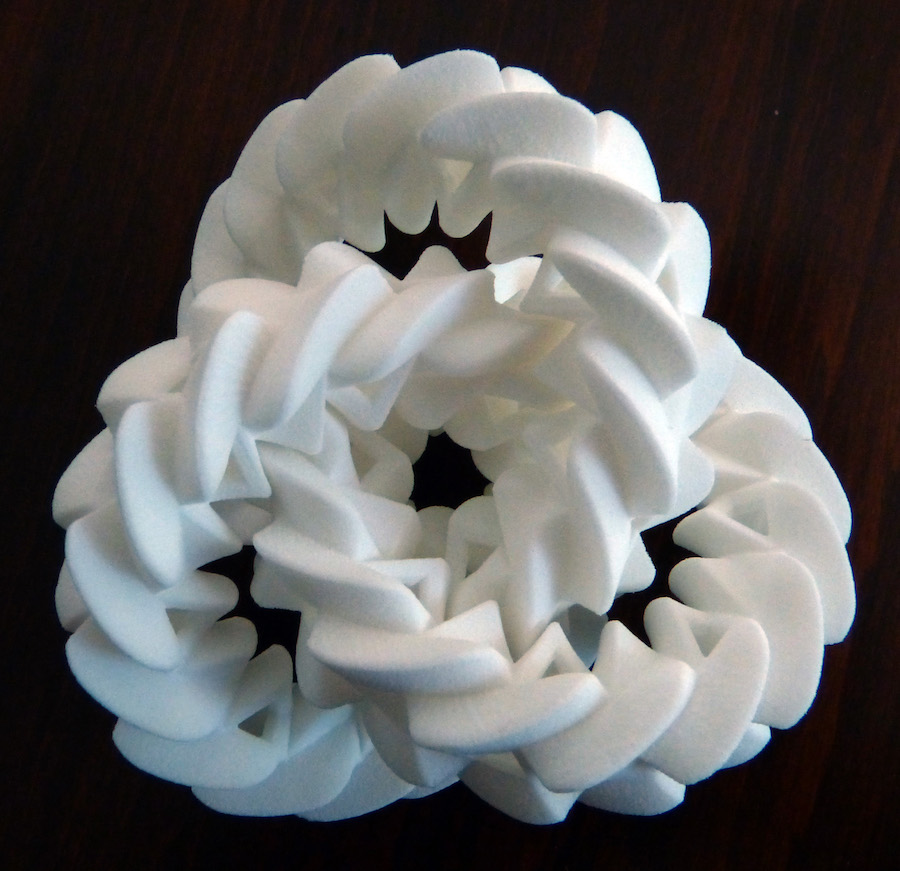
\includegraphics[width=0.65\textwidth]{mechanic trefoil}
    \caption{Mechanisch model van gekoppelde knoopwervel, visueel analoog van traagheid.}
\end{figure}



\begin{figure}[h!]
    \centering
    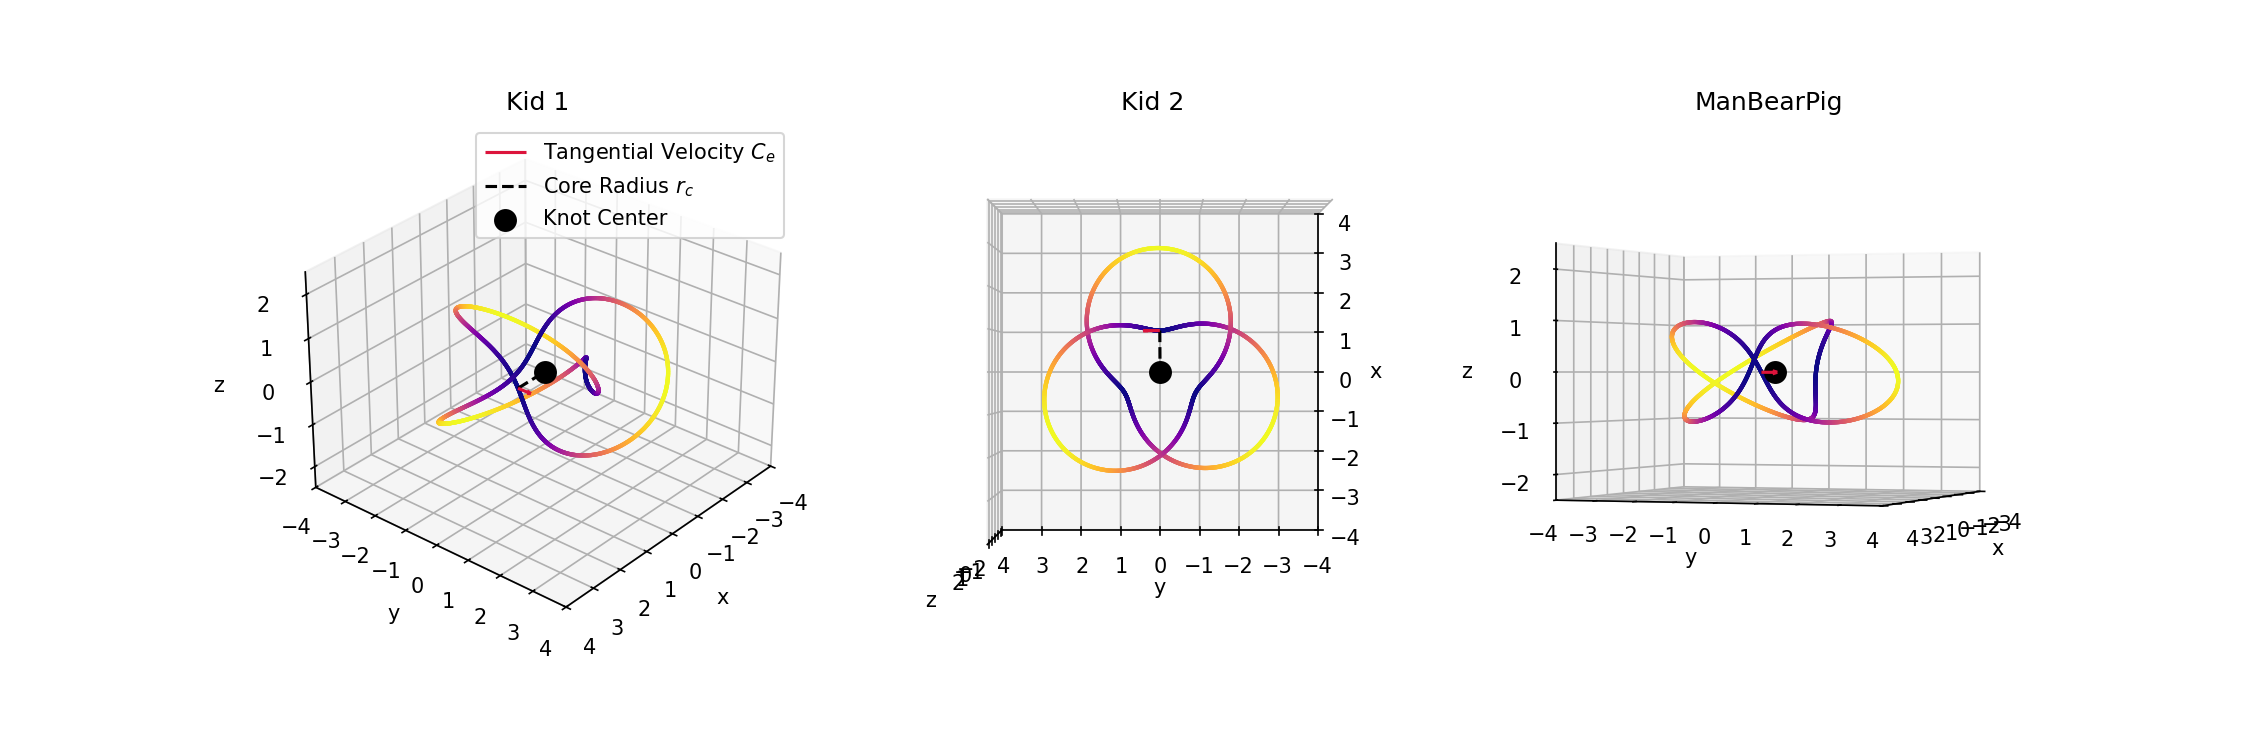
\includegraphics[width=0.95\textwidth]{vortex_knot_diagram.png}
    \caption{Annotatie kernstraal $r_c$ en swirlrichting $C_e$.}
\end{figure}